\section{Fokker-Planck equation}
Derivation of the Folkee-Planck equation for a general Langevin equation (Itô prescription)

We start from a stochastic process defined vie the Langerin equation (Itô)\
(1) \quad $d x(t)=\mu(x(t), t) d t+\sigma(x(t), t) d B(t)$
where $x(0)=x_{0}$ (or a generic initial $P D F$ ). $B(t)$ is a standard Brownion process.
An alternative way to write eq. (1) is the "psendo-equation"
(2) $\dot{x}=\mu(x, t)+\sigma(x, t) \xi(t)$

Where $\langle\xi(t)\rangle=0$ and $\left\langle\xi\left(t^{\prime}\right) \xi(t)\right\rangle=\delta\left(t^{\prime}-t\right)$. We used the sugfestive relation " $\frac{d B}{d t}=\xi$ ", even though this is only a formal, notational expression.

Eq. (1) defines the process $x(t)$ so we can use the ep. to generate as many trajectories as we wish. Let us assume that we have generated a lage number $N$ of poths from time $t=0$ to $t=T>0$. How con we colulate the probability that $x(t)$ gets a value between $x$ and $x+\Delta x$ (a PDF) at time $t$ ?

From the computational point of view this is relatively eosy :
\begin{center}
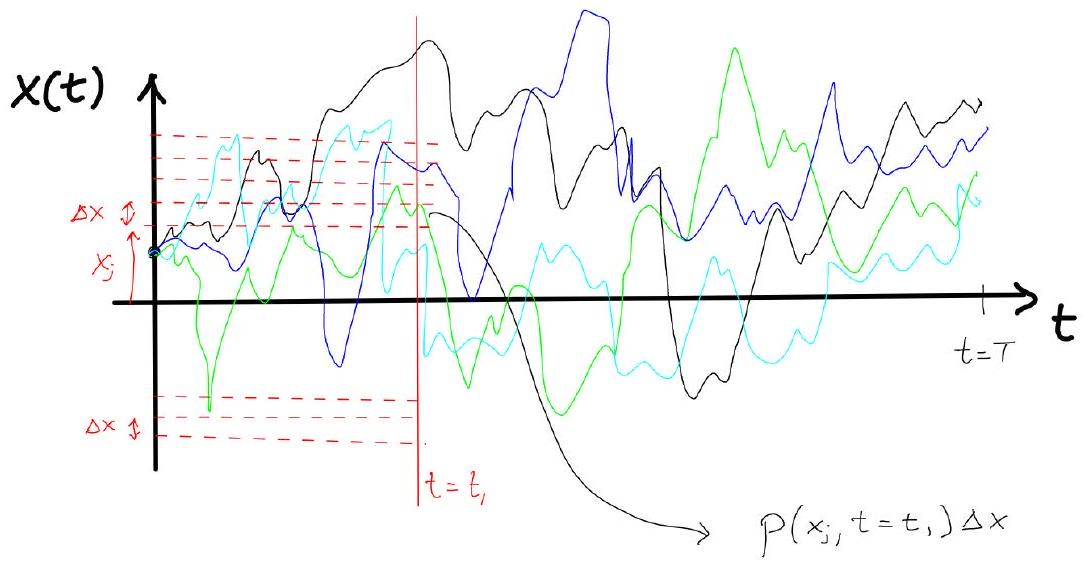
\includegraphics[width=0.8\textwidth]{2025_10_17_15d569b79a40ed74679eg-02}
\end{center}

$$
N=4
$$

We have to count how mony paths foll in the interval $[x, x+\Delta x)$ at time $t=t_{1}$ as $x$ veries in the domain of definition of the process $x(t)$.
If we use the indicator function, $I$, defined as

$$ I(a, A)= \begin{cases}
1 & a \in A \ 0 & a \notin A
\end{cases}
$$

then we colculate numerically $P(x, t)$ as
(3) $P\left(x_{j}, t=t_{1}\right) \Delta x=\lim _{N \rightarrow \infty} \frac{1}{N} \sum_{1}^{N} I\left(x^{i}\left(t_{1}\right),\left[x_{j}, x_{j}+\Delta x\right)\right)$ for any $x_{j}$ and verious $t$.

Where $x_{j}=j \Delta x$ and $j=j_{\min }, j_{\min }+1, \ldots j_{\max }-1, j_{\max }$ (uniform mesh). For example, if the process was Brownion, then $P(x, t)$ would be very well approximated by a Gaussion distribution with zero mean and varience $t$, as we saw before. Notice that if we say $x_{j}=x, t=t$, and toke the limit $\Delta x \rightarrow 0$, then
(36) $P(x, t)=\lim _{N \rightarrow \infty} \frac{1}{N} \sum_{i}^{N} \delta\left(x-x_{i}(t)\right)$ es $\lim _{\Delta x \rightarrow 0} \frac{I\left(x^{i}(t),[x, x+\Delta x)\right)}{\Delta x}=\delta\left(x-x_{i}(t)\right)$

From the theoretical point of view we want to find out an equation for $P(x, t)$ which gives the PDF of the process $x(t)$. If we are interested in the statistics of the process, then $P(x, t)$ gives all the information we need, for we con
calculate all averages we wont (all moments)
(even though it is not guaranteed that from the PDF we con exactly reconstruct the process $x(t)$ pathwise).
Actually, we con calculate the average of any "sufficiently regular" function $f$.
Let's assume that $f$ has compact support in $\mathbb{R}$ and is twice-differentiable, mamely $f \in C_{c}^{2}(\mathbb{R})$.
Then we con calculate $\langle f(x(t))\rangle$, avarage of $f$ over the process. If we are given $N$ indep. zealizations of $x(t)$, then as $N \rightarrow \infty \langle f(x(t))\rangle=\lim _{N} \frac{1}{N} \sum_{i}^{N} f\left(x_{i}(t)\right)=\lim _{N} \frac{1}{N} \sum_{i}^{N} \int d x f(x) \delta\left(x-x_{i}(t)\right)=$


\begin{equation*}
=\int d x f(x) \lim _{N} \frac{1}{N} \sum_{i}^{N} \delta\left(x-x_{i}(t)\right) \stackrel{\downarrow}{=} \int d x f(x) p(x, t) \tag{35}
\end{equation*}


Hence

$$ \text { (5) } \quad \frac{d}{d t}\langle f(x(t))\rangle \equiv \int \dot{p}(x, t) f(x) d x $$

Here $\langle\cdots\rangle$ means that the average of $f$ has to be calculated over the whole set of trajectories of the process $x(t)$. We now diserentize the procen in time and Taylor-expand the function $f(x)$ :
(6) $f(x(t+\Delta t))=f(x(t))+\Delta x f^{\prime}(x(t))+\frac{\Delta x^{2}}{2} f^{\prime \prime}(x(t))+$ h.o.t.
where from ef. (1) we get
(7) $\quad \Delta x \equiv x(t+\Delta t)-x(t)=\mu(x(t), t) \Delta t+\sigma(x(t), t) \Delta B(t)$

Therefore from (6) $\Delta f \equiv f(x(t+\Delta t))-f(x(t))$

$$ \begin{aligned}
\Delta f & =f^{\prime}(\mu \Delta t+\sigma \Delta B)+\frac{1}{2} f^{\prime \prime}(\mu \Delta t+\sigma \Delta B)^{2}+\text { h.o.t. } \\ & =f^{\prime}(\mu \Delta t+\sigma \Delta B)+\frac{1}{2} f^{\prime \prime}\left(\mu^2\Delta t^2 + 2 \mu \sigma \Delta t \Delta B+\sigma^{2} \Delta B^{2}\right)+\text { h.o.t. }
\end{aligned}
$$

We now consider the average of each term:
a) $\left\langle f^{\prime} \sigma \Delta B\right\rangle=\left\langle f^{\prime} \sigma\right\rangle\langle\Delta B\rangle=0$

Itô prescription
b) $\left\langle f^{\prime \prime} \mu \sigma \Delta t \Delta B\right\rangle=\left\langle f^{\prime \prime} \mu \sigma\right\rangle \Delta t\langle\Delta B\rangle=0$
c) $\frac{1}{2}\left\langle f^{\prime \prime} \sigma^{2} \Delta B^{2}\right\rangle=\frac{1}{2}\left\langle f^{\prime \prime} \sigma^{2}\right\rangle\left\langle\Delta B^{2}\right\rangle=\frac{1}{2}\left\langle f^{\prime \prime} \sigma^{2}\right\rangle \Delta t$ Itô preser. IMPORTANT!
all remaining terms are $O\left(\Delta t^{2}\right)$.
Therefore eq. (5) con be re-written as limit
(9) $\quad \lim _{\Delta t \rightarrow 0}\left\langle\frac{\Delta f}{\Delta t}\right\rangle=\left\langle f^{\prime} \mu\right\rangle+\frac{1}{2}\left\langle f^{\prime \prime} \sigma^{2}\right\rangle$

$$ \begin{aligned}
& =\int d x p(x, t)\left[f^{\prime}(x) \mu(x, t)+\frac{1}{2} f^{\prime \prime}(x) \sigma^{2}(x, t)\right]
\end{aligned}
$$ 

As $f \in C_{c}^{2}(\mathbb{R})$ we can integrate by parts and safely assume that $f, f^{\prime}$ and $f^{\prime \prime} \rightarrow 0$ as $|x|$ is large enough. Hence
(10)

$$ \int d x p(x, t) \mu(x, t) \frac{\partial f}{\partial x} \stackrel{\downarrow}{=}-\int d x f(x) \frac{\partial}{\partial x}(p \mu)
$$ 
twice integrated by parts

$$ \int d x p(x, t) \frac{\sigma^{2}(x, t)}{2} \frac{\partial^{2} f}{\partial x^{2}}=\frac{1}{2} \int d x f(x) \frac{\partial^{2}}{\partial x^{2}}\left(\sigma^{2}(x) p\right) $$

and

$$ \frac{d}{d t}\langle f(x)\rangle=\int d x f(x) \frac{\partial}{\partial t} p(x, t) $$

Thus from eps. (9) and (10) and because $f \in C_{c}^{2}(\mathbb{R})$ but arbitrary we end up with
(11) $\quad \frac{\partial}{\partial t} p(x, t)=-\frac{\partial}{\partial x}[\mu(x, t) p(x, t)]+\frac{1}{2} \frac{\partial^{2}}{\partial x^{2}}\left[\sigma^{2}(x, t) p(x, t)\right]$

This is the forward Fokker-Planck equation corresponding to the process defined in el. (1) with the Itop prescription. The FP ep. (11) con be used to derive the propagoton of the process $x(t)$; we need just to solve it with the imitial condition $P\left(x, t_{0}\right)=\delta\left(x-x_{0}\right)$, namely, this gives the fundamental solution $P\left(x, t \mid x_{0}, t_{0}\right)$. If we can colculate $P(x, t)$ then we can find all the averages (= statistics) of the procen defined by the Langevin ef. (1). Notice that ep. (11) is a deterministic and linear PDE for $p(x, t)$.

Eq. (11) can also be written as

$$ \frac{\partial p}{\partial t}=-\frac{\partial J}{\partial x}(x, t) $$

(12)

$$ J(x, t) \equiv \mu(x, t) p(x, t)-\frac{1}{2} \frac{\partial}{\partial x} \sigma(x, t) p(x, t) $$

where $J(x, t)$ is the flux at $x$ at time $t$. This form shows that, if the process $x(t)$ is defined in the domain $D \subseteq \mathbb{R}$, then

$$ \frac{\partial}{\partial t} \int_{D} p(x, t) d x=-\int_{D} \frac{\partial J}{\partial x} d x=-\left.J\right|_{x \in \partial D} $$

where $2 D$ is the boundary of $D$. If there is no "leakage" of probability, then $\left.J\right|_{x \in \partial D}=0$ and we con set $\int_{D} p(x, t) d x=1$ at any time $t$ (conservation of probability).

Notice that ep. (11) must be equipped with boundary conditions if the process $x(t)$ is defined in given domain $D \subset \mathbb{R}$. For instance, if $D=\mathbb{R}^{+}$one has to define what happens at $x=0$ at any time $t>0$.

\begin{itemize}
  \item Absorbing boundary conditions require: $\left.p(x, t)\right|_{x \in 20}=0, \forall t$
  \item Reflecting boundory conditions require: $\left.J(x, t)\right|_{x \in \partial D}=0 \quad \forall t$ N3: these are the correct conditions when $\left.\sigma(x, t)\right|_{x \in \partial D}>0 \quad \forall t$ Equilibrium solution of the Fokker-Planct equation Let us assume that $\mu(x, t)=\mu(x)$ and $\sigma(x, t)=\sigma(x)$ and also that the propogator defined by ef. (11) reaches an equilibrium solution, nancely
\end{itemize}

$$ \lim _{t \rightarrow \infty} p\left(x, t \mid x_{0}, t_{0}\right)=p^{s t}(x) $$

what is the form of $p^{s t}(x)$ ? From. ey. (11) $\partial_{t} p^{s t}=0$ implies

$$ -\frac{\partial}{\partial x}\left(\mu(x) p^{t}-\frac{1}{2} \frac{\partial}{\partial x} \sigma^{2}(x) p^{s t}\right)=0 $$

hence

$$ J^{s t}(x)=\mu(x) p^{s t}-\frac{1}{2} \frac{\partial}{\partial x} \sigma^{2}(x) p^{s t}=\text { const } \text { for any } x \text {. } $$

If there is no current at any point $x \in D$, we obtain the equilibrium solution (with reflecting boundory conditions at $\partial D$ )

$$ \mu(x) p^{s t}(x)=\frac{1}{2} \frac{\partial}{\partial x}\left(\sigma^{2}(x) p^{s t}(x)\right) $$

Since

$$ \begin{aligned}
& \frac{2 \mu}{\sigma^{2}}\left(\sigma^{2} p^{s t}\right)=\frac{\partial}{\partial x}\left(\sigma^{2} p^{s t}\right) \\ & \sigma^{2} p^{s t}=\text { const } e^{\int^{x} \frac{2 \mu}{\sigma^{2}} d y}
\end{aligned}
$$ 

hence the equilibrium solution has the form (ref.bound. at $x_{m}, x_{m}$ )
(13)

$$ p^{s t}(x)=\frac{1}{2} \frac{1}{\sigma^{2}(x)} e^{2 \int_{x_{m}}^{x} \frac{\mu(y)}{\sigma^{2}(y)} d y} \quad x_{m} \leq x \leq x_{\mu} $$

where $z \equiv \int_{x_{m}}^{x_{M}} \frac{d x}{\sigma^{2}(x)} e^{2 \int_{x_{m}}^{x} \frac{\mu(y)}{\sigma^{2}(y)} d y}<\infty$, and $\int_{x_{m}}^{x_{M}} p^{s t}(x) d x=1$.
Some caveats:
Notice that ep. (13) may not exist. Also we have not proved that it is unique, nor that it can be reached by some initial conditions.
Eq. (13) is only the form one expects if indeed an equilibrium solution exists. Indeed, it does not depend on initial conditions and the equilibrium sol. is only determined by $\mu$ and $\sigma$ (and the refe.b.c.), so it is an intrinsic property of the system which is not tuned by how we imitially prepare the system.

The Ornstein- Unleubeck proces
As a rimple application of what we have studied we investigate the O-U process. From previous lectures we know that it is defined by the SDE
(14) $\left\{\begin{array}{lll}d x=-\mu x d t+\sigma d B(t) & \text { or } & \dot{x}=-\mu x+\sigma \xi_{t} \\ x(0)=x_{0} & \left(\left\langle\xi_{t}\right\rangle=0,\left\langle\xi_{t} \xi_{t^{\prime}}\right\rangle=\delta\left(t-t^{\prime}\right)\right)\end{array}\right.$

Where $\mu, \sigma$ are positive constants and $B$ is the B.m. From e. II (I) we obtain the F.P. equation for the PDF:
(15) $\dot{p}=-\frac{\partial}{\partial x}[(-\mu x) p]+\frac{\sigma^{2}}{2} \frac{\partial^{2}}{\partial x^{2}} p$

The equilibrium distribution of (15) (from ep. (13)) is

$$ p^{s t}(x) \propto e^{-\frac{2}{\sigma^{2}} \int^{x} \mu y d y}=e^{-\frac{\mu}{\sigma^{2}} x^{2}} $$

(16)

$$ p^{s t}(x)=\sqrt{\frac{\mu}{\pi \sigma^{2}}} e^{-\frac{\mu}{\sigma^{2}} x^{2}} $$

which is a Gaussian distribution with mean 0 and variance $\frac{\sigma^{2}}{2 \mu}$.
Exercige: Show that the equation for the verionce that ane gets from ep. (14) is the some that one gets from ep. (15). Verify that at stationarity the value is $\sigma^{2} / 2 \mu$.

Indeed on con colculate the evolution in time of the PDF.

By taking the Fourier transform of ep. (15) (which gives you the time evolution of the characteristic function of the process) one finds the full solution (which is the propogetor of the $0 .-U$. pocess)
(17) $p\left(x, t \mid x_{0}, s\right)=\sqrt{\frac{\mu}{\pi \sigma^{2}\left(1-e^{-\mu(t-s)}\right)}} e^{-\frac{\mu}{\sigma^{2}} \frac{\left(x-x_{0} e^{-\mu(t-s)}\right)^{2}}{1-e^{-\mu(t-s)}}}$
for which $P\left(x, s \mid x_{0}, s\right)=\delta\left(x-x_{0}\right)$. Another way to find the solution is to stort from the ansots

$$ p(x, t) \propto e^{-A x^{2}+x B+C} $$

sub this into ey. (15) and find $A, B$ and $C$ as a function of $t$ and $x_{0}$. The normalization and the imitial condition finally give q.(17).

All these findings can be generalized to the case

$$ \dot{p}=-\frac{\partial}{\partial x}[(\alpha-\mu x) p]+\frac{\sigma^{2}}{2} \frac{\partial^{2}}{\partial x^{2}} p $$

and also to the multidimensional O.-U. procen (Gardiner, p. 105).

\section*{Porticle in a large medium}
We study the anotion of a particle suspended in a loye (fhid) medium. The particle should be much bigger than those of the medium but small enough to change position and momentum when calliding with the medium's particles. The surrounding medium is a heat bath at Hermal equilisrium with a const. temperoture $T$ (homgeneous and isotropic).
If we had to account fir all interactions of the suspended (mesoscopic) porticle of mass $m$, we would write
\begin{center}
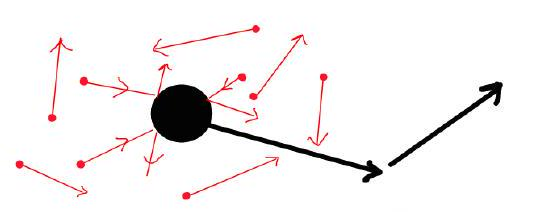
\includegraphics[width=0.5\textwidth]{2025_10_17_15d569b79a40ed74679eg-10}
\end{center}

\begin{itemize}
  \item Lluid porticles at tem
  \item mesoscopic porticle
\end{itemize}


\begin{equation*}
m \ddot{\vec{x}}(t)=\vec{F}_{\text {ext }}(\vec{x}(t))+\sum_{i}^{N} i \vec{F}\left(\vec{x}(t)-\vec{x}_{i}(t)\right) \tag{18}
\end{equation*}


where $\vec{F}_{\text {ext }}$ is an external face that may (or not) be described by a potentiol, where the i-th porticle exerts on susp. particle e force $\bar{F}\left(\bar{x}-\overline{x_{i}}\right)$. As $N \simeq N_{A}$ (Avogadro number), it is pointlen to integrate ey. (18). It's more appropriate to treat the medium porticles in an effective way, like an effective force acting an the susp. porticle. Thus

$$ \sum_{i}^{N} i \vec{F}\left(\vec{x}(t)-\vec{x}_{i}(t)\right) \simeq \vec{F}_{\text {aven }}+\vec{F}_{\text {moise }} $$

As the mesoscopic particle callides with the smaller fluid partills there is viscons domping generated by the callisions in the fhid. If the velocity of the perticle isn't too lage we con approximate $\vec{F}_{\text {aver }}=-\gamma \vec{v}=-\gamma \dot{\vec{x}}, \gamma$ being the demping coefficient. From hydrodynomics, we con set $\gamma=6 \pi \eta R$, $\eta$ being the viscasity and $R$ the Browmion porticle's roolins.
We also assume that all fhid portilles have independent mestions and every porticle's movement is independent on different time intervals (if not too small).

Also, if there is a time interval $\tau$ (much smaller of time intervals of obsensation st) large enough that in any two successive time intends $r$ the motions of the mesosegric particle con be considered independent events, then we can effectivaly approximate $\vec{F}_{\text {moise }}$ as a stachastic process that is proportional to a Brownian motion.
For simplicity, let's consider the 1 -d cose with no extended forces. So from (18)


\begin{equation*}
m \ddot{x}=-\gamma \dot{x}+\sigma \xi(t) \tag{19}
\end{equation*}

where $\langle\xi\rangle=0$ and $\left\langle\xi(t) \xi\left(t^{\prime}\right)\right\rangle=\delta\left(t-t^{\prime}\right)$. Notice that this process is non-Morkovian. Let's multiply both sides by $x$, then

$$ m x \frac{d}{d t} \dot{x}=-\gamma x \dot{x}+\sigma x \xi_{t} $$

Since $\frac{d^{2}}{d t^{2}} x^{2}=2\left(\dot{x}^{2}+x \ddot{x}\right)$, then

$$ \frac{m}{2} \frac{d^{2}}{d t^{2}}\left(x^{2}\right)-m \dot{x}^{2}=-\frac{\gamma}{2} \frac{d}{d t}\left(x^{2}\right)+6 x \xi_{t} $$

Take the average of both sides and use Iton presaiption:

$$ \frac{m}{2} \frac{d^{2}}{d t^{2}}\left\langle x^{2}\right\rangle-2 \cdot \frac{m}{2}\left\langle\dot{x}^{2}\right\rangle=-\frac{\gamma}{2} \frac{d}{d t}\left\langle x^{2}\right\rangle $$

Because of the equiportition theorem in classical mechanics

$$ \frac{m}{2}\left\langle\dot{x}^{2}\right\rangle=\frac{1}{2} k_{B} T $$

$k_{B}$ : Boltz mom's constant
hence T: absolute temperature


\begin{equation*}
m \frac{d^{2}}{d t^{2}}\left\langle x^{2}\right\rangle+\gamma \frac{d}{d t}\left\langle x^{2}\right\rangle=2 k_{B} T \tag{19b}
\end{equation*}

Define $y(t)=\frac{d}{d t}\left\langle x^{2}\right\rangle$, then (19b) becomes

$$ m \dot{y}+\gamma y=2 k_{B} T $$

Whose solution is $y(t)=c e^{-\frac{\gamma}{m} t}+\frac{2 k_{B} T}{\gamma}$ and $c$ is an arbitrary constant.
In suspended porticles $\frac{m}{\gamma} \simeq 10^{-8} \mathrm{sec}$, which on temporal scales of observation is a tiny time. Hence for $t \gg 10^{-8} \mathrm{sec}, y \simeq \frac{2 k B T}{\gamma}$ and

$$ \frac{d}{d t}\left\langle x^{2}\right\rangle \simeq \frac{2 k_{B} T}{\gamma} $$

so (20) $\left\langle x^{2}(t)\right\rangle-\left\langle x_{0}^{2}\right\rangle=\frac{2 k_{B} T}{\gamma} t$ for $t \gg 10^{-8} \mathrm{sec}$
limeas increase of the mean square deviation.
This seminds us of the simple Brownion motion. Indeed, let's stort from
(21) $\dot{x}=\sqrt{2 D} \xi_{t}$ or $d x=\sqrt{2 D} d B(t)$
which leads to the diffusive equation

$$ \frac{\partial}{\partial t} p(x, t)=D \frac{\partial^{2}}{\partial x^{2}} p(x, t) \quad D \text { is diffusivity } $$

From (21) $x(t)=x_{0}+\sqrt{2 D} B(t)$ and
(22)

$$ \left\langle x^{2}\right\rangle=\left\langle x_{0}^{2}+2 x_{0} \sqrt{2 D} B(t)+2 D B(t)^{2}\right\rangle=x_{0}^{2}+2 D t $$
diffusion law

By componing op. (20) and (22), we obtain
(23) $D=\frac{k_{B} T}{\gamma}$ Einstein's relation

This is the finst and simplest example of fluctuation-dissipation theorem.

\section*{Obs:}
\begin{enumerate}
  \item Eq. (23) tells how we should choose the diffusivity if we wont to interpret physically the menoscopic particle as a free perticle within an equilibrium therund both at temper. T.
  \item $D$ does not depend on initial conditions, or the nature of interactions between the fluid particles and the Brownion particle, all we need to know is that the system is at equilibrium in a system where general behaviou is summariged by the damping constant $\gamma$. (We coptured some universal behovion here!).
  \item From the diffusion law in ef. (22) one con measure $D$, hence We can give an estimete of $k_{B}$ and $N_{A}=\frac{R}{k_{B}}$, the Avogedro number ( $R$ is the gas constant). This is what Einstein suggested in his 1905 pioneering wast on Brownian motion.
  \item This interputation is stroightforward if we start from ep. (19) with $\sigma=\sqrt{2 \gamma k_{B} T}$ and then take the limit $\frac{m}{\gamma} \rightarrow 0$ which is colled the overdomped limit:
\end{enumerate}

$$ \frac{m}{\gamma} \ddot{x}=-\dot{x}+\frac{\sqrt{2 \gamma k_{B} T}}{\gamma} \xi_{t} \xrightarrow{m / \gamma \rightarrow 0} \quad \dot{x}=\sqrt{2 \frac{k_{B} T}{\gamma}} \xi_{t} $$

overdomped Longevia equation

\section*{Connection with Statistical Mechanics}
From stat. Mech. we know haw to colculate the PDF that a porticle hos momentum $\vec{p}$ and position $\vec{x}$ when it is locoted within an extemal potential $U(\bar{x})$ and is surnounded by a heat bott at equilibrium at temperature $T$. This is
(24) $\mathbb{P}(\vec{x}, \vec{p})=\frac{1}{z} e^{-\beta\left(\frac{\bar{p}^{2}}{2 m}+U(\bar{x})\right)} \quad \begin{gathered}\text { Boltzmanm's weight } \\ \beta=\frac{1}{k_{B} T}\end{gathered}$

where $m$ is the mon of the porticle, $z=\int d \vec{p} \int d \vec{x} \mathbb{P}(\bar{x}, \bar{p})=\left(2 \pi m k_{B}\right)^{3 / 2} z_{0}$ is the total portition function and $z$. the reduced one. From ep. (21) one gets the PDF to dosewe the porticle at $\vec{x}$ at equilibrium regardles of its momentum. This is


\begin{equation*}
w(\\vec{x})=\\frac{1}{z_{0}} e^{-\\beta U(\\vec{x})} \tag{25}
\end{equation*}

Can we commect these classical results with the theory we have developed so far? Yes! We will do it for a 1-d system, but the generalization is simple and direct. Let's stort from ep. (19) where now we assume that the particle experiences a conservative external force $f_{\text {ext }}=-\partial_{x} U(x)$, being $U(x)$ the potential of the face. We also assume that the Brownion porticle is at equil. with the heat both at temper. $T$, so $\sigma=\sqrt{2 \gamma k_{B} T}$ :
(26)

$$ m \ddot{x}=-\partial_{x} U(x)-\gamma \dot{x}+\sqrt{2 \gamma k_{B} T} \xi_{t} $$

In the overdomped limit ( $\frac{m}{\gamma} \rightarrow 0$ ) we get


\begin{equation*}
\dot{x}=-\frac{\partial_{x} U}{\gamma}+\sqrt{2 D} \xi_{t} \quad D=\frac{k_{B} T}{\gamma} \tag{23}
\end{equation*}

or

$$ d x=-\frac{1}{\gamma} \partial_{x} U d t+\sqrt{2 D} d B(t) $$

\section*{(27)}
The consesponding Folken-Plonck equation of 9.27 is


\begin{equation*}
\frac{\partial}{\partial t} p(x, t)=-\frac{\partial}{\partial x}\left[-\frac{1}{\gamma}\left(\partial_{x} U\right) p\right]+D \frac{\partial^{2}}{\partial x^{2}} p \tag{28}
\end{equation*}

You can check that the equilibrium distribution of eq. (28) is given by (see ep. (13))
(29) $P_{\text {ep }}(x) \propto e^{-\frac{1}{D \gamma} \int^{x} \partial_{y} U(y) d y} \propto e^{-\frac{1}{D \gamma} U(x)}$
but $D \gamma=k_{B} T$, so e. P. P. $(x)$ and $w(x)$ in eq. (25) are exactly the some.

\section*{Obs :}
\begin{enumerate}
  \item Notice that we could have fixed $D=\frac{k_{B} T}{\gamma}$ by imposing that QP. (29) and (25) are the same! This is zemorkable and shows that the value of $D$ does not depend on the potential $U$, which is somehow unexpected and confirms the universolity of Einstein's velotion in es. (23).
  \item Notice that if $U(x)=\frac{1}{2} k x^{2}$, then ep. (27) reads
\end{enumerate}

$$ d x=-\frac{k}{\gamma} x d t+\sqrt{2 \frac{k_{B} T}{\gamma}} d B(t) $$

\begin{center}
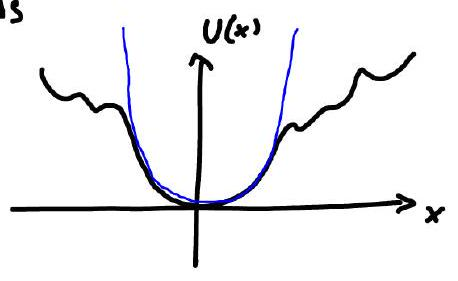
\includegraphics[width=\textwidth]{2025_10_17_15d569b79a40ed74679eg-15}
\end{center}
which is an $0 .-U$ process with the equilibrium distribution:

$$ p_{\text {eq }}(x)=\sqrt{\frac{k \beta}{2 \pi}} e^{-\frac{1}{2} \beta k x^{2}} $$

Browmian particle in contact with a heat bath at equilibrium and forced by a harmomic potential We stort from ep. (26) where $U(x)=\frac{1}{2} k x^{2}$ and $\sigma=\sqrt{2 \gamma k_{B} T}$ :
(30) $m \ddot{x}=-k x-\gamma \dot{x}+\sqrt{2 \gamma k_{B} T} \xi_{t}$
where $x$ is the porticle coordinate at time $t$, $m$ its mon, $g$ the friction coefficient as before.
Eq. (30) is a lineor ey. and con be solved even though the process is non-Morkovian beconse of $\ddot{x}$. We write

$$ x(t)=x_{c}(t)+x_{\xi}(t) $$

where $x_{c}$ sotisfies the homogeneous $\varphi .( \xi=0)$ with $x_{c}(0)=x_{0}$ and $\dot{x}_{c}=v_{0}$. $x_{\xi}$ satisfies the in-homog. ep. with $x_{\xi}(0)=0$ and $\dot{x}_{\xi}(0)=0$.
Show that

$$ x_{c}(t)=A e^{-\gamma_{0} t} \sin (\Omega t)+B e^{-\gamma_{0} t} \cos (\Omega t) $$

where $A, B$ are arbitrony constants and

$$ \gamma_{0}=\frac{\gamma}{2 \mu}, \quad \Omega=\omega_{0}^{2}-\gamma_{0}^{2}, \quad \omega_{0}^{2}=\frac{k}{m} ;
$$ 

and

$$ x_{\xi}(t)=\sqrt{2 \gamma k_{0} T} \frac{1}{m \Omega_{0}} \int_{0}^{t} e^{-\gamma \cdot(t-s)} \sinh [\Omega(t-s)] \xi(s) d s $$

$\underbrace{}_{d B(s)}$
Prove that

$$ \left\langle x^{2}(t)\right\rangle=\frac{2 \gamma k_{B} T}{m^{2} \Omega_{0}^{2}} \int_{0}^{t} e^{-2 \gamma_{0}(t-s)} \sinh ^{2}[\Omega(t-s)] d s \underset{t \rightarrow \infty}{\longrightarrow} \frac{k_{B} T}{m \omega_{0}^{2}} $$

\begin{itemize}
  \item Con you interpect this result from the physical point of view?
  \item Repeat the colculations for the velocity $v(t)=\dot{x}$
  \item Con you colculate $\langle x(t) x(s)\rangle$ ? If necessory, fix $|t-s|$ and take the limit $t \rightarrow \infty, s \rightarrow \infty$.
\end{itemize}